\documentclass[tikz]{standalone}
\usepackage{float}              % [H]
\usepackage{graphicx}           % (pdf, png, jpg, eps)
\usepackage{tikz}
\usepackage{pgfplots}
\usepackage{pgfplotstable}
\usepackage{siunitx}
\usepackage{currfile}
\usepackage{ifthen}
\pgfplotsset{compat=1.17}
\usepgfplotslibrary{polar}
\usepgfplotslibrary{colorbrewer}
\usetikzlibrary{calc}
% 
\def\datapath{../../__PATH__} % relative to build path
\directlua0{
   pdf.setinfo ("/Path: (__PATH__)")
 }
% 
\pgfplotsset{%
  colormap/cividis/.style={colormap={cividis}{[1pt]
    rgb(0pt)=(0.00000000, 0.13511200, 0.30475100);
    rgb(25pt)=(0.25974000, 0.30512000, 0.42281000);
    rgb(50pt)=(0.48514100, 0.48245100, 0.47038400);
    rgb(75pt)=(0.73242200, 0.67736400, 0.42571700);
    rgb(100pt)=(0.99573700, 0.90934400, 0.21777200);
}}}
%  
../../thesis/content/parameters.tex
% 
\newlength{\width}
\newlength{\height}
\setlength{\width}{13.87303cm} %5.462 inch
\setlength{\height}{22.37076cm} %8,807 inch
\def\radiusvalue{0.5}
% 
\def\deltax{4.2}
\def\deltay{4.2}
% 
\begin{document}
% 
% \foreach \omegavalues/\psivalues [count=\pp] in {{30.0,60.0,90.0}/{0.3,0.6,0.9}}{
\foreach \omegavalues/\psivalues [count=\pp] in {{30.0,60.0,90.0}/{0.3,0.6,0.9},{0.0,10.0,20.0,30.0,40.0,50.0,60.0,70.0,80.0,90.0}/{0.1,0.2,0.3,0.4,0.5,0.6,0.7,0.8,0.9}}{
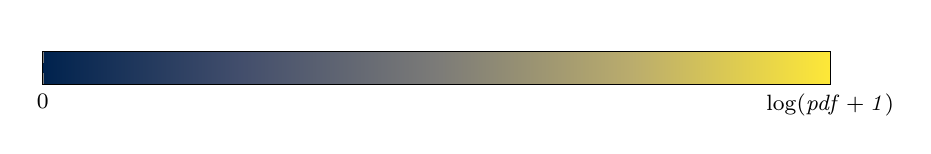
\begin{tikzpicture}
% 
\pgfplotsset{every tick label/.append style={font=\footnotesize}}
% 
\foreach \omegavalue [count=\i] in \omegavalues {
\foreach \psivalue [count=\j] in \psivalues {
\begin{scope}[shift={(\j*\deltax,-\i*\deltay)}, local bounding box=\i\j]
  \begin{scope}[local bounding box=bb]
    \begin{polaraxis}[
        width=5cm, height=5cm,
        xtick={0,90,...,270},
        xticklabels={\rotatebox[origin=c]{-90}{$\SI{0}{\degree}$},%
                     $\SI{90}{\degree}$,%
                     \rotatebox[origin=c]{90}{$\SI{180}{\degree}$},%
                     $\SI{270}{\degree}$,%
                     },
        extra x ticks={45,135,...,315},
        % extra x tick labels={,,,},
        extra x tick labels={$\SI{45}{\degree}$,%
                             $\SI{135}{\degree}$,%
                             $\SI{225}{\degree}$,%
                             $\SI{315}{\degree}$},
        ytick={60,30},
        yticklabels={$\SI{30}{\degree}$,$\SI{60}{\degree}$},
        yticklabel style=white,
        tickwidth=0,
        separate axis lines,
        y axis line style= { draw opacity=0 },
        ymin=0, ymax=90,
        axis on top=true,
        % colorbar,
        % colorbar style={
        %   ytick={0,1},
        %   yticklabels={$0$,$\log(\mathit{pdf+1})$},
        % },
        colormap/cividis,
      ] 
      \addplot [%
          matrix plot*,
          point meta=explicit,]
        table[meta expr={ln(\thisrowno{2}+1)}]
          {\datapath/hist/cube_stats_p_\psivalue_o_\omegavalue_r_\radiusvalue.dat};
      \coordinate (A) at (0,90);
      \coordinate (B) at (180,90);
      \coordinate (C) at (\omegavalue,90);
      \coordinate (D) at (\omegavalue+180,90);
      \coordinate (CC) at (0,0);
    \end{polaraxis}
    % 
    \draw[white, very thick, dashed] (A) -- (B);
    \draw[white, very thick, dashed] (C) -- (D);
    % 
  \end{scope}
  \begin{scope}[overlay]
    \pgfmathparse{int(round(\psivalue*10))*10}
    \ifthenelse{\i=1}{\node[anchor=south, xshift=-0.2ex] at (bb.north) {$\modelPsi = \SI{\pgfmathresult}{\percent}$};}{}
    \ifthenelse{\j=1}{\node[anchor=south, xshift=-0.2ex, rotate=90] at (bb.west) {$\modelOmega = \SI{\omegavalue}{\degree}$};}{}
  \end{scope}
  % center
  \path[] ($(CC)-(2.7,0)$) -- ($(CC)+(2.7,0)$);
  \path[] (CC) -- ($(CC)+(0,2.7)$);
\end{scope}
}}
% 
\begin{scope}[shift={(current bounding box.south)}, xshift=-5cm,]
  \begin{axis}[%
    hide axis,
    scale only axis,
    height=0pt, width=0pt,
    xmin=0, xmax=1, ymin=0, ymax=1,
    colormap/cividis,
    colorbar horizontal,
    point meta min = 0,
    point meta max = 1,
    colorbar style={
        width=10cm,
        height=0.42cm,
        xticklabel style={tick label style={font=\footnotesize}},
        xtick={0,1},
        xticklabels={$0$,$\log(\mathit{pdf+1})$},
    }]
  \end{axis}
\end{scope}
% 
\end{tikzpicture}
}
% 
\end{document}
